\documentclass[11pt,a4paper]{article}

\usepackage{geometry}
 \geometry{
 a4paper,
 total={150mm,237mm},
 left=30mm,
 top=30mm,
 }

% cf. http://tex.stackexchange.com/questions/50182/subtitle-with-the-maketitle-page
\usepackage{titling}
\newcommand{\subtitle}[1]{%
  \posttitle{%
    \par\end{center}
    \begin{center}\large\textbf{#1}\end{center}
    \vskip0.5em}%
}

\usepackage{color}
\usepackage{graphicx}
\usepackage{subcaption}

\usepackage[utf8]{inputenc}
\usepackage[lf]{venturis} %% lf option gives lining figures as default; 
\usepackage[T1]{fontenc}
\usepackage{csquotes}
\usepackage[UKenglish,german]{babel}

\usepackage{fancyvrb}

\widowpenalty10000  % http://tex.stackexchange.com/questions/4152/how-do-i-prevent-widow-orphan-lines
\clubpenalty10000

\title{The SysSon Platform}
\subtitle{Technical Report TR-2016-10-1\\Institute of Electronic Music and Acoustics, Graz\\(Status: in progress)}
\author{Hanns Holger Rutz}
% \date{09-Feb-2016}
\date{October 2016}

% cf. https://tex.stackexchange.com/questions/94126/change-font-to-only-section-and-subsection-of-my-document
%\usepackage{titlesec}
%\titleformat{\chapter}[display]
%  {\fontfamily{pag}\selectfont\huge\bfseries}
%  {\chaptertitlename\ \thechapter}
%  {20pt}
%  {\Huge}
%\titleformat{\section}
%  {\fontfamily{pag}\selectfont\bfseries\Large}
%  {\thesection}
%  {1em}
%  {}
%\titleformat{\subsection}
%  {\fontfamily{pag}\selectfont\bfseries\Large}
%  {\thesection}
%  {1em}
%  {}

\usepackage[backend=biber,authordate]{biblatex-chicago} % citereset=chapter
%\usepackage[backend=biber,natbib,isbn=false,useprefix=true,sorting=ydnt]{biblatex-chicago} % citereset=chapter
\addbibresource{all.bib} % add a bib-reference file
\addbibresource{rutz.bib} % add a bib-reference file

% warning: https://tex.stackexchange.com/questions/313477/
% \usepackage{csquotes}

\usepackage{tabularx}
% cf. https://tex.stackexchange.com/questions/84400/table-layout-with-tabularx-column-widths-502525
\newcolumntype{s}{>{\hsize=1cm}X}

% says you should load after babel and fontspec
\usepackage[shrink=10, babel=true]{microtype}	% http://tex.stackexchange.com/questions/141852/latex-allows-line-break-between-concluding-em-dash-and-comma-before-a-new-sub-cl/141854#141854

% has to come first for full scale TeX voodoo bullcrap
\usepackage{hyperref}
% get rid of the horrible coloured boxes around links
\hypersetup{
    colorlinks,%
    citecolor=black,%
    filecolor=black,%
    linkcolor=black,%
    urlcolor=black
}
% has to come after frickin hyperref
\VerbatimFootnotes

\newcommand{\todo}[1]{\colorbox{yellow}{\textsc{todo}: #1}}

\newcommand{\quot}[1]{\guillemotleft {#1}\guillemotright}

\newcommand{\worktitle}[1]{\textit{#1}}

\newcommand{\workentry}[2]{\vspace{7.5pt}\noindent\textbf{#1} (#2)}
\newcommand{\workentrySel}[2]{\vspace{7.5pt}\noindent\textbf{#1}$*$ (#2)}

\newcommand{\figref}[1]{Fig.~\ref{#1}}

\newcommand{\software}[1]{\textit{#1}}

\newcommand{\sysson}[0]{SysSon}
\newcommand{\syssonVersion}[0]{1.8.0}
\newcommand{\syssonVersionS}[0]{1.8.0-SNAPSHOT}

\newcommand{\artefacts}[0]{\textsc{Artefacts:}}
\newcommand{\assessment}[0]{\textsc{Assessment:}}

\begin{document}
% \begin{titlepage}
\maketitle
\selectlanguage{UKenglish}
\thispagestyle{empty}
\newpage
\section{First Sonification Scenario}

Following a project meeting on 16-Sep-2016, it was decided that the first scenario or template to work out is to look at QBO (quasi-biennial-oscillation) and ENSI (El Niño), using two sets of measured temperature data.\footnote{%
A different scenario discussed are "stratospheric sudden warmings", which happen around the poles in 30\,km altitude. The sudden jumps in temperature of up to 70 degrees happen within  weeks, and proceed from top to bottom.%
}

We had worked with QBO sonification already in one of the previous workshops. One usually selects a specific range in the altitudes and rather equatorial coordinates (e.g. +/- 10 degrees). Longitudes are often averaged, but we will try to also look at longitudinal movements.

QBO and ENSO interact with each other in that strong amplitudes in ENSO (lower altitudes) are connected with the inverse phenomena in the QBO (higher altitudes). It would thus be interesting to be also able to sonically compare the two.

\subsection{Data Files}

\begin{itemize}
\item {\small \Verb!5x5-climatology_2001-05-01_2016-05-01_RO_OPSv5.6.2_L2b_no_METOP_no_TerraSAR-X.nc!}\\A high-resolution file with 5x5 latitude/longitude grid, 600 altitude levels, and over 180 months (10.1\,GB)
\item {\small \Verb!5x30-climatology_2001-05-01_2016-05-01_RO_OPSv5.6.2_L2b_no_METOP_no_TerraSAR-X.nc!}\\A slightly lower resolution file with 5x50 latitude/longitude grid (1.7\,GB)
\end{itemize}

Initial problems:
%
\begin{itemize}
\item File selection filter did not know about HDF files (previously only NetCDF files were used); \textbf{Result: fixed}
\item Heatmap plots somehow fail to gather the statistics of the data. \textbf{Result: It is just running very slowly (c. 12 minutes).}
\item After stats finally complete, data is useless because we don't have fill value information, and apparently something different from NaN is used. \textbf{Result: Converted file to use NaNs}
\item Date format not recognised. Time unit is "seconds since 1990-01-01T00:00:00", somehow that is not correctly parsed. \textbf{Result:  fixed}
\item The dimensions "Latitude" and "Longitude" are not correctly recognised, because the map-overlay option is not shown. \textbf{Result: fixed}
\end{itemize}
%
We might:
%
\begin{itemize}
\item look into updating the NetCDF library and drop Java 6 support. New artifact is called \Verb!netcdf4! and latest version is 4.6.6. This might improve performance. \textbf{Result: no speed improvement}
\item introduce a simple table view, so one can quickly browse the data numerically.
\item create a preference item to \emph{disable} automatic removal of cache upon application quit.
\item we also need to be able to adjust the cache size, because the 1.7 GB files produces already a 230 KB stats cache, therefore we will easily transcend the default cache size of 1 MB.
\end{itemize}
%
After further inspection, fill values are correctly stored and found as -1e-10. Strangely stats show a max of 2.4e22 and a mean of 5.1e14. For example, for dry temperature those values appear in time index 90 and altitude indices 5 to 8. Here a "spike" of 4.49e23 in altitude index 5 declines towards index 8, and at index 9 the data is in the normal range again. We thus need to first preprocess that file and replace out-of-range values with the defined fill value. \textbf{Result: fixed by converting data.}

\todo{continue here}

\begin{figure}
% \centering
\begin{subfigure}[b]{1.0\textwidth}%
\centering
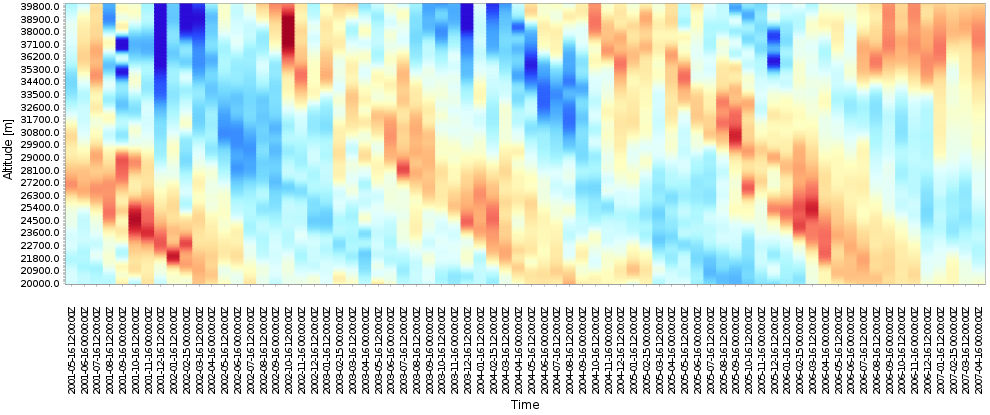
\includegraphics[scale=0.45,trim=2mm 0 1mm 1mm]{figures/ta_anomalies_mean.jpg}
\caption{Using monthly mean}
\label{fig:anomaly-mean}
\end{subfigure}
\begin{subfigure}[b]{1.0\textwidth}%
\centering
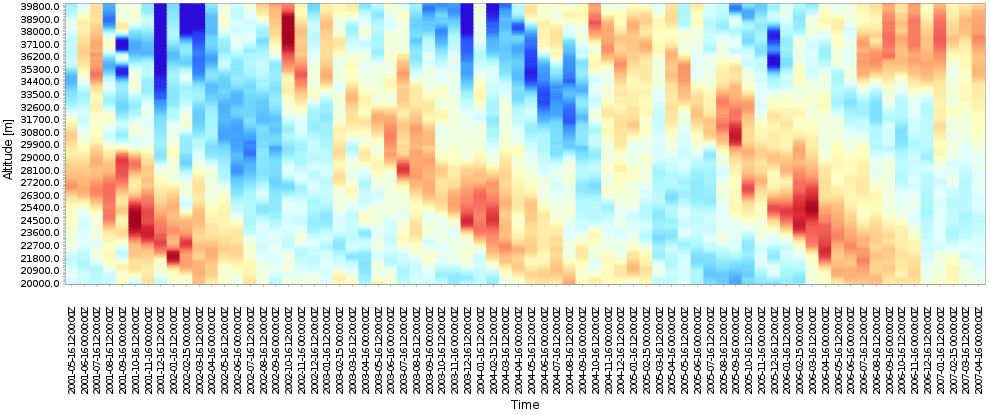
\includegraphics[scale=0.45,trim=2mm 0 1mm 1mm]{figures/ta_anomalies_median.jpg}
\caption{Using monthly median}
\label{fig:anomaly-mean}
\end{subfigure}
\caption{Temperature anomalies calculated with different norms.}
\label{fig:anomaly-calc}
\end{figure}

Plots: 105 degrees west, 2.5 degrees south.

%\begin{figure}[h]
%\centering
%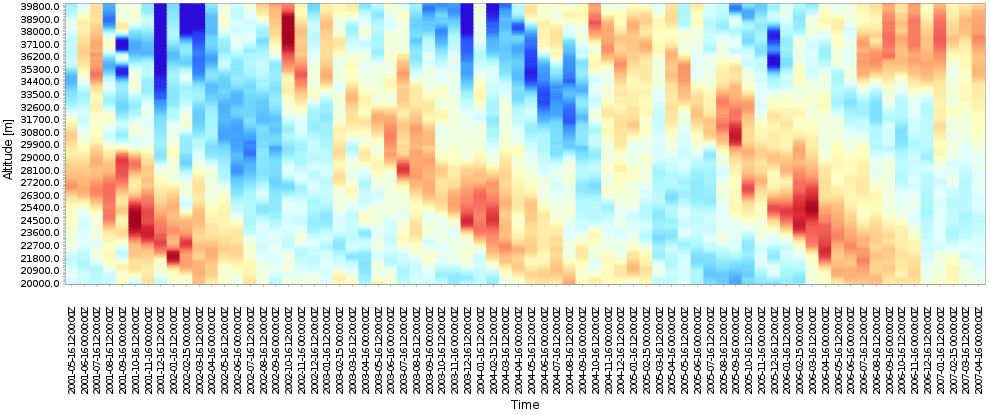
\includegraphics[scale=0.5]{figures/ta_anomalies_median.jpg}
%\caption{Temperature anomalies calculated based on monthly median.}
%\label{fig:anomaly-mean}
%\end{figure}

% \printbibliography

\end{document}